\documentclass{article}
\usepackage[utf8]{inputenc}
\usepackage{mdframed}
\usepackage{float}

\title{18-05-2012}

\date{May 2021}

\usepackage{natbib}
\usepackage{graphicx}
\DeclareUnicodeCharacter{2212}{-}
\begin{document}

\maketitle

\section{Elliptic Curves}
\subsection{Introduction}
\begin{figure}[h]
	\begin{center}
  		\includegraphics[width=1 \textwidth,]{images/intro.png}
 	\end{center}
 	\label{init}
\end{figure}

\begin{figure}[h]
	\begin{center}
  		\includegraphics[width=1 \textwidth,]{images/ecc.png}
 	\end{center}
 	\label{init}
\end{figure}

\subsection{How to Compute with Elliptic Curves}
We start by giving a short introduction to the mathematical concept of elliptic
curves, independent of their cryptographic applications. ECC is based on the generalized
discrete logarithm problem. Hence, what we try to do first is to find a cyclic group on which we can build our cryptosystem. Of course, the mere existence of a
cyclic group is not sufficient. The DL problem in this group must also be computationally
hard, which means that it must have good one-way properties.
We start by considering certain polynomials (e.g., functions with sums of exponents
of x and y), and we plot them over the real numbers.

Example 9.1. Let’s look at the polynomial equation ${x2+y2 = r2}$ over the real numbers
R. If we plot all the pairs (x,y) which fulfill this equation in a coordinate system, we obtain a circle as shown in Fig. 9.1.

\begin{figure}[h]
	\begin{center}
  		\includegraphics[width=0.5 \textwidth,]{images/fig9-1png.png}
  		\caption{Plot of all points (x, y) which fulfill the equation ${a^2 + b^2 = r^2 }$over R }
 	\end{center}
 	\label{init}
\end{figure}

Example 2 . A slight generalization of the circle equation is to introduce coefficients
to the two terms x2 and y2, i.e., we look at the set of solutions to the equation
a · x2 +b · y2 = c over the real numbers. It turns out that we obtain an ellipse, as shown in Figure 2.

\begin{figure}[h]
	\begin{center}
  		\includegraphics[width=0.5 \textwidth,]{images/fig9-2.png}
  		\caption{Plot of all points (x, y) which fulfill the equation ${ax^2 + b y^2 = c }$ over R }
 	\end{center}
\end{figure}
\subsection{Definition of Elliptic Curves}

From the two examples above, we conclude that we can form certain types of curves
from polynomial equations. By “curves”, we mean the set of points (x,y) which are solutions of the equations. For example, the point (x = r,y = 0) fulfills the equation
of a circle and is, thus, in the set. The point (x = r/2,y = r/2) is not a solution to the
polynomial ${x^2+y^2 = r^2}$ and is, thus, not a set member. An elliptic curve is a special
type of polynomial equation. For cryptographic use, we need to consider the curve
not over the real numbers but over a finite field. The most popular choice is prime
fields GF(p), where all arithmetic is performed modulo a prime p.

 
\begin{figure}[h]
	\begin{center}
  		\includegraphics[width= 0.8 \textwidth,]{images/def9.1.1.png}
 	\end{center}
\end{figure}

The definition of elliptic curve requires that the curve is nonsingular. Geometrically
speaking, this means that the plot has no self-intersections or vertices, which
is achieved if the discriminant of the curve \textbf{-}${16(4a^3+27b^2)}$ is nonzero.
For cryptographic use we are interested in studying the curve over a prime field
as in the definition. However, if we plot such an elliptic curve over ${Z_p}$, we do not get
anything remotely resembling a curve. However, nothing prevents us from taking an
elliptic curve equation and plotting it over the set of real numbers.



We notice several things from this elliptic curve plot.1 First, the elliptic curve
is symmetric with respect to the x-axis. This follows directly from the fact that for
all values xi which are on the elliptic curve, both ${yi = \sqrt {x_1^3 + a x_i + b}}$ and ${yi =  - \sqrt{x_1^3 + a x_i + b}}$ are solutions. Second, there is one intersection with the x-axis.
This follows from the fact that it is a cubic equation if we solve for y = 0 which has
one real solution (the intersection with the x-axis) and two complex solutions (which
do not show up in the plot). There are also elliptic curves with three intersections
with the x-axis.
We now return to our original goal of finding a curve with a large cyclic group,
which is needed for constructing a discrete logarithm problem. The first task for
finding a group is done, namely identifying a set of elements. In the elliptic curve
case, the group elements are the points that fulfill Eq. (9.1).

\begin{figure}[h]
	\begin{center}
  		\includegraphics[width= 0.8 \textwidth,]{images/example.png}
 	\end{center}
\end{figure}

\addvspace{1cm}

Note: Notice that in the above examples the expression ${f(x, y) = y^2 - x^3 - 7}$ is the same but the
elliptic curves are different. To avoid such ambiguities the notation E(GF(q)) or E(Fq) is
often used in the literature. That is to say, the goal of this notation is to remember that
the coordinates x, y belong to the finite Galois field GF(q).\\
 
Notice that the number of points in E is less than ${2 |GF(q)|}$. The number of points on E is
usually denoted as ${|E|}$ or \#E.
 
 For q a prime number I will write: 
 $${f(x,y) = 0 (mod q)}$$

 which indicates that we are computing modulo q.


\subsection{Group Operations on Elliptic Curves}

 \begin{mdframed}
\section{from slide}
The important fact about elliptic curves is that two points (x1, y1), (x2, y2) of E can be
“added” to get a third point (x3, y3) of E: 
$$ { (x_1, y_1) + (x_2,y_2) = (x_3, y_3)}$$ 
The set E endowed with the operation is commutative group. Moreover:
\begin{enumerate}
    \item such “addition” of points on E is computationally feasible.
    \item as consequence of 1) any cryptographic algorithm based on the discrete logarithm can be
adapted to work on a elliptic curve.
    \item usually the tradeoff key dimension vs. security level of adaptations as 2) are highly better
than the originals.
\end{enumerate}
\end{mdframed}

Let’s denote the group operation with the addition symbol “+”. “Addition” means
that given two points and their coordinates, say P = (x1,y1) and Q = (x2,y2), we
have to compute the coordinates of a third point R such that: 

$$ { P + Q = R}$$
$$ { (x_1, y_1) + (x_2,y_2) = (x_3, y_3)}$$ 

As we will see below, it turns out that this addition operation looks quite arbitrary.
Luckily, there is a nice geometric interpretation of the addition operation if we
consider a curve defined over the real numbers. For this geometric interpretation,
we have to distinguish two cases: the addition of two distinct points (named point
addition) and the addition of one point to itself (named point doubling).

\textbf{Point Addition P+Q} This is the case where we compute R = P+Q and ${P \ne Q}$. The construction works as follows: Draw a line through P and Q and obtain a
third point of intersection between the elliptic curve and the line. Mirror this third
intersection point along the x-axis. This mirrored point is, by definition, the point R.
Figure 9.4 shows the point addition on an elliptic curve over the real numbers.

\textbf{Point Doubling P+P} This is the case where we compute P+Q but P=Q. Hence,
we can write R = P+P = 2P. We need a slightly different construction here. We draw the tangent line through P and obtain a second point of intersection between
this line and the elliptic curve. We mirror the point of the second intersection along
the x-axis. This mirrored point is the result R of the doubling. Figure 9.5 shows the doubling of a point on an elliptic curve over the real numbers. \\

\begin{figure}[h]
	\begin{center}
  		\includegraphics[width= 0.8 \textwidth,]{images/fig9.4.png}
 	\end{center}
\end{figure}

\begin{figure}[h]
	\begin{center}
  		\includegraphics[width= 0.8 \textwidth,]{images/fig9.5.png}
 	\end{center}
\end{figure}

You might wonder why the group operations have such an arbitrary looking form.
Historically, this tangent-and-chord method was used to construct a third point if
two points were already known, while only using the four standard algebraic operations
add, subtract, multiply and divide. It turns out that if points on the elliptic
curve are added in this very way, the set of points also fulfill most conditions necessary
for a group, that is, closure, associativity, existence of an identity element and
existence of an inverse.
Of course, in a cryptosystem we cannot perform geometric constructions. However,
by applying simple coordinate geometry, we can express both of the geometric constructions from above through analytic expressions, i.e., formulae. As stated
above, these formulae only involve the four basic algebraic operations. These operations
can be performed in any field, not only over the field of the real numbers. In particular, we can take the curve equation from above, but we now
consider it over prime fields GF(p) rather than over the real numbers. This yields
the following analytical expressions for the group operation.

\begin{figure}[h]
	\begin{center}
  		\includegraphics[width= 0.8 \textwidth,]{images/addition.png}
 	\end{center}
\end{figure}

Note that the parameter s is the slope of the line through P and Q in the case of
point addition, or the slope of the tangent through P in the case of point doubling.
Even though we made major headway towards the establishment of a finite group,
we are not there yet. One thing that is still missing is an identity (or neutral) element
${\sigma}$ such that: $${P + \sigma = P}$$

for all points P on the elliptic curve. It turns out that there isn’t any point (x,y) that
fulfills the condition. Instead we define an abstract point at infinity as the neutral
element ${\sigma}$. This point at infinity can be visualized as a point that is located towards
“plus” infinity along the y-axis or towards “minus” infinity along the y-axis.
According the group definition, we can now also define the inverse \textbf{-}P of any
group element P as:
${\sigma}$ such that: $${P + (-P) = \sigma}$$

The question is how do we find −P? If we apply the tangent-and-chord method
from above, it turns out that the inverse of the point P = (xp,yp) is the point  ${-P =
(x_p, −y_p)}$, i.e., the point that is reflected along the x\textbf{-}axis. Figure 9.6 shows the point
P together with its inverse. Note that finding the inverse of a point P = (xp,yp) is
now trivial. We simply take the negative of its y coordinate. In the case of elliptic
curves over a prime field GF(p) (the most interesting case in cryptography), this is
easily achieved since \textbf{-}${yp \equiv (p - y_p)}$ (mod p)  , hence
    
$${ - P = (x_p, p - y_p)}$$

Now that we have defined all group properties for elliptic curves, we now look at
an example for the group operation. \\
We consider a curve over the small field ${Z_1{_7}}$:

\begin{figure}[H]
	\begin{center}
  		\includegraphics[width= 0.8 \textwidth,]{images/ex9.6.png}
 	\end{center}
\end{figure}

$${E : y^2 \equiv x^3 + 2x + 2 ( mod 17 )}$$  

We want to double the point P = (5, 1) 

\begin{figure}[h]
	\begin{center}
  		\includegraphics[width= 0.8 \textwidth,]{images/eq.png}
 	\end{center}
\end{figure}

For illustrative purposes we check whether the result 2P = (6,3) is actually a point
on the curve by inserting the coordinates into the curve equation:

\begin{figure}[h]
	\begin{center}
  		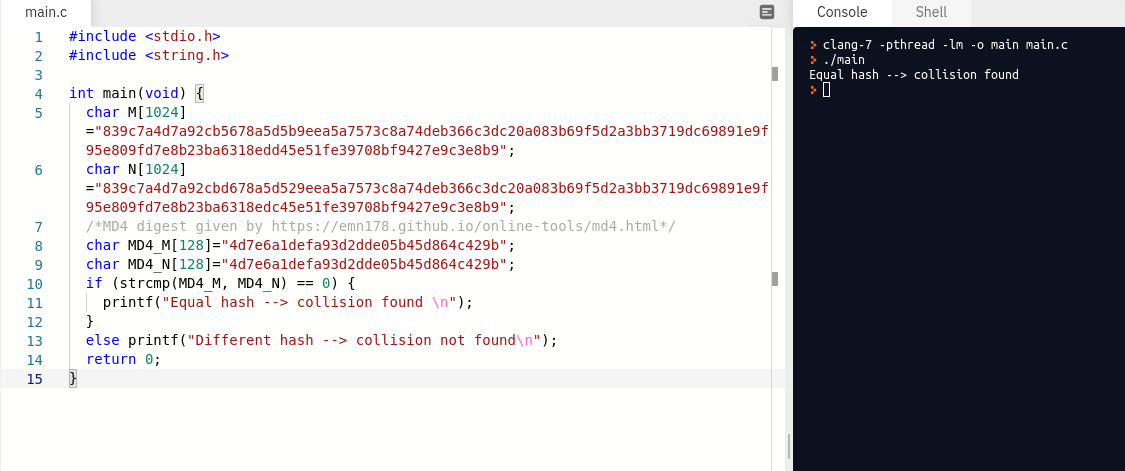
\includegraphics[width= 0.8 \textwidth,]{images/sol.png}
 	\end{center}
\end{figure}

summary: it is clear that by knowing points P and Q and using algorithm you can compute a point called P + Q $\rightarrow$ tag. 

From math: you should prove that this + indeed an "abelian group operation"\\

See also the exercise done by the professor in week11 page n.2 with points P(6,6) and Q(15,16).
\end{document}